\pdfminorversion=4
\documentclass[compress,
mathserif,wide,%red,
%handout
]{beamer}

\usepackage{amsmath,amsfonts,bm,bbm,comment}
\usepackage{latexsym,tabularx,amscd}
\usepackage{etex} 
\usepackage{algorithm}
\usepackage[noend]{algorithmic}
\usepackage{subfigure}
\usepackage{url}
%\usepackage{multimedia}
\usepackage{hyperref}
\usepackage{skull}
%\usepackage{enumitem}
%\usepackage{movie15}

\usepackage{multirow}
\usepackage{cancel}

%\usepackage{ulem}
\usepackage{lmodern}
\usepackage{array} 
\usepackage{etoolbox}
\usepackage{caption}
\usepackage[normalem]{ulem}

\usepackage{mathtools}

\usepackage[space]{grffile}

\usepackage{tikz}
\usetikzlibrary{shapes.arrows}
\usetikzlibrary{arrows,positioning}
\usepackage{pgfplots}
%\usetikzlibrary{pgfplots.groupplots}

\tikzset{
    myarrow/.style={
        draw,
        fill=black,
        single arrow,
        minimum height=6ex,
        single arrow head extend=1ex
    }
}


\newcommand{\vertiii}[1]{{\left\vert\kern-0.25ex\left\vert\kern-0.25ex\left\vert #1 
    \right\vert\kern-0.25ex\right\vert\kern-0.25ex\right\vert}}

\newcommand{\vertiiibig}[1]{{\big\vert\kern-0.25ex\big\vert\kern-0.25ex\big\vert #1 
    \big\vert\kern-0.25ex\big\vert\kern-0.25ex\big\vert}}

\newcommand{\vertiiiplain}[1]{{\vert\kern-0.25ex\vert\kern-0.25ex\vert #1 
    \vert\kern-0.25ex\vert\kern-0.25ex\vert}}



\usepackage{dsfont}
\DeclareMathOperator{\ind}{\mathds{1}}  % Indicator


\newcommand{\abs}[1]{\left|#1\right|}

\mode<presentation>

\usetheme{Madrid}
% other themes: AnnArbor, Antibes, Bergen, Berkeley, Berlin, Boadilla,
% boxes, CambridgeUS, Copenhagen, Darmstadt, default, Dresden,
% Frankfurt, Goettingen, Hannover, Ilmenau, JuanLesPins, Luebeck,
% Madrid, Maloe, Marburg, Montpellier, PaloAlto, Pittsburg, Rochester,
% Singapore, Szeged, classic

% \usecolortheme{lily} 
% color themes: albatross, beaver, beetle, crane, default, dolphin,
% dov, fly, lily, orchid, rose, seagull, seahorse, sidebartab,
% structure, whale, wolverine

% \usefonttheme{serif} 
% font themes: default, professionalfonts, serif, structurebold,
% structureitalicserif, structuresmallcapsserif

%\usefonttheme[onlymath]{serif}
%\usefonttheme[onlylarge]{structuresmallcapsserif} 
  
%\useoutertheme[subsection=false]{smoothbars}
% outer themes:
% default,infolines,miniframes,smoothbars,sidebar,split,shadow,tree,smoothtree
%\useinnertheme{rectangles}
\beamertemplatenavigationsymbolsempty

% \definecolor{fore}{RGB}{249,242,215}
% \definecolor{back}{RGB}{51,51,51}
% \definecolor{title}{RGB}{255,0,90}
% \setbeamercolor{titlelike}{fg=title}
% \setbeamercolor{normal text}{fg=fore,bg=back}
% \setbeamercovered{transparent}
  % or whatever (possibly just delete it)
%\beamertemplatenavigationsymbolsempty

\usepackage[english]{babel}
\usepackage[latin1]{inputenc}
% or whatever
%\usepackage{comicsans} 
%\renewcommand{\sfdefault}{comic} 
%\usepackage{mathptmx}
%\mathversion{bold}
%\usepackage{helvet}
%\usepackage{courier}

%\usepackage[T1]{fontenc}
% Or whatever. Note that the encoding and the font should match. If T1
% does not look nice, try deleting the line with the fontenc.


%%%% Figures %%%%%


\newcommand{\LectureFigs}{../Figures}


\definecolor{bluegray}{rgb}{0.15,0.20,0.40}
\definecolor{bluegraylight}{rgb}{0.35,0.40,0.60}
\definecolor{gray}{rgb}{0.3,0.3,0.3}
\definecolor{lightgray}{rgb}{0.7,0.7,0.7}
\definecolor{brightblue}{rgb}{0.1,0.4,0.7}
\definecolor{darkblue}{rgb}{0.1,0.1,0.6}
\definecolor{darkgreen}{rgb}{0.0,0.5,0.2}
\definecolor{orange}{rgb}{0.7,0.3,0}

\def \captioncolor { }

\setbeamertemplate{itemize item}{{\color{black}$\bullet$}}
\setbeamertemplate{itemize subitem}{{\color{black}$\circ$}}
\setbeamertemplate{frametitle}[default][center]
\setbeamerfont{frametitle}{series=\bfseries}
\addtobeamertemplate{frametitle}{\vskip1ex}{ \vspace{0.5em} \hrule}
\setbeamercolor{frametitle}{fg=,bg=}

\setbeamertemplate{theorems}[numbered]
\setbeamertemplate{caption}[numbered]
\setbeamertemplate{algorithm}[numbered]

\numberwithin{theorem}{subsection}
\numberwithin{equation}{subsection}
\numberwithin{figure}{subsection}
\numberwithin{algorithm}{subsection}


%\setbeamerfont{page number in head/foot}{size=\scriptsize}
\setbeamertemplate{footline}[frame number]
\setbeamercolor{page number in head/foot}{fg=black}
\setbeamersize{text margin left=2em,text margin right=2em}

\setbeamertemplate{footline}
{
    %\hspace{3em} \insertshorttitle \hfill \insertframenumber / \inserttotalframenumber\hspace{3em}
    \hspace{3em} \insertshorttitle \hfill \insertsubsectionnumber-\insertframenumber \hspace{3em}
    \vspace{1.5em}
}

\definecolor{babyblueeyes}{rgb}{0.63, 0.79, 0.95}
\definecolor{bleudefrance}{rgb}{0.19, 0.55, 0.91}
\definecolor{matlabPlotBlue}{rgb}{0.25, 0.58, 0.8}
\definecolor{matlabPlotOrange}{rgb}{0.855, 0.324, 0.098}



\captionsetup[figure]{labelfont={color=black}}

\AtBeginEnvironment{lemma}{%
  \setbeamercolor{block title}{fg=black,bg=babyblueeyes}
  \setbeamercolor{block body}{fg=black,bg=}
  \setbeamerfont*{block title}{series=\bfseries}
}

\AtBeginEnvironment{theorem}{%
  \setbeamercolor{block title}{fg=black,bg=babyblueeyes}
  \setbeamercolor{block body}{fg=black,bg=}
  \setbeamerfont*{block title}{series=\bfseries}
}

\AtBeginEnvironment{corollary}{%
  \setbeamercolor{block title}{fg=black,bg=babyblueeyes}
  \setbeamercolor{block body}{fg=black,bg=}
  \setbeamerfont*{block title}{series=\bfseries}
}

\AtBeginEnvironment{fact}{%
  \setbeamercolor{block title}{fg=black,bg=babyblueeyes}
  \setbeamercolor{block body}{fg=black,bg=}
  \setbeamerfont*{block title}{series=\bfseries}
}

\AtBeginEnvironment{definition}{%
  \setbeamercolor{block title}{fg=black,bg=babyblueeyes}
  \setbeamercolor{block body}{fg=black,bg=}
  \setbeamerfont*{block title}{series=\bfseries}
}

\newenvironment<>{varblock}[2][.9\textwidth]{%
  \vspace{-1em}
  \begin{center}
  \begin{minipage}{#1}
  %\setlength{\textwidth}{#1}
  \begin{actionenv}#3%
    \def\insertblocktitle{#2}%
    \par%
    \usebeamertemplate{block begin}}
  {\par%
    \usebeamertemplate{block end}%
  \end{actionenv}
  \end{minipage}
  \end{center}
}


\newcommand\blankfootnote[1]{%
  \let\thefootnote\relax\footnotetext{#1}%
  \let\thefootnote\svthefootnote%
}


%%%%%
\newcommand{\bb}{\bm b}
\newcommand{\bZ}{\bm Z}
\newcommand{\bC}{\bm C}
\newcommand{\cU}{{\cal U}}
\newcommand{\bR}{{\bm R}}
\newcommand{\bi}{{\bm i}}
\newcommand{\bS}{{\bm S}}
\newcommand{\cE}{{\cal E}}
\newcommand{\cF}{{\cal F}}
\newcommand{\bk}{{\bm k}}
\newcommand{\bu}{{\bm u}}
\newcommand{\bx}{{\bm x}}
\newcommand{\bA}{{\bm A}}
\newcommand{\bh}{{\bm h}}
\newcommand{\by}{{\bm y}}
\newcommand{\bI}{{\bm I}}
\newcommand{\ba}{{\bm a}}
\newcommand{\bw}{{\bm w}}
\newcommand{\bPhi}{{\bm \Phi}}
\newcommand{\bX}{{\bm X}}
\newcommand{\bY}{{\bm Y}}
\newcommand{\bM}{{\bm M}}
\newcommand{\be}{{\bm e}}
\newcommand{\bs}{{\bm s}}
\newcommand{\bB}{{\bm B}}
\newcommand{\bW}{{\bm W}}
\newcommand{\bN}{{\bm N}}
\newcommand{\bU}{{\bm U}}
\newcommand{\bV}{{\bm V}}
\newcommand{\bP}{{\bm P}}
\newcommand{\bH}{{\bm H}}
\newcommand{\bSigma}{{\bm \Sigma}}
\newcommand{\bL}{{\bm L}}



\newcommand{\bv}{\bm v}
\newcommand{\eps}{\epsilon}
\newcommand{\vf}{\varphi}
\newcommand{\de}{\delta}
\newcommand{\<}{\langle}
\renewcommand{\>}{\rangle}
\newcommand{\goto}{\rightarrow}
\newcommand{\argmin}{\mbox{argmin}}
\newcommand{\argmax}{\mbox{argmax}}
\newcommand{\Ave}{\mathop{\rm Ave}\nolimits}
\newcommand{\sgn}{\mbox{sgn}}
\newcommand{\cN}{\mathcal{N}}
\newcommand{\cR}{\mathcal{R}}

\def\C{{\mathbb{C}}}
\def\R{{{\mathbb{R}}}} %seemed too large in subscripts, so I changed --JW 
\def\P{{\hbox{\bf P}}}
\def\Z{{{\mathbb{Z}}}}
\def\T{{\hbox{\bf T}}}


\newcommand{\cA}{\mathcal{A}}
\newcommand{\cP}{\mathcal{P}}
\newcommand{\cD}{\mathcal{D}}
\newcommand{\cL}{\mathcal{L}}
\newcommand{\shrink}{\text{shrink}}


\newcommand{\Obs}{\Omega_{\text{obs}}}


\renewcommand{\P}{\operatorname{\mathbb{P}}}
\newcommand{\E}{\operatorname{\mathbb{E}}}

% Linear algebra macros
%\newcommand{\vct}[1]{#1}
%\newcommand{\mtx}[1]{#1}
\newcommand{\vct}[1]{\bm{#1}}
\newcommand{\mtx}[1]{\bm{#1}}
%\newcommand{\mtx}[1]{\mathsfsl{#1}}

\newcommand{\transp}{T}
\newcommand{\adj}{*}
\newcommand{\psinv}{\dagger}
\newcommand{\lspan}[1]{\operatorname{span}{#1}}

\newcommand{\range}{\operatorname{range}}
\newcommand{\colspan}{\operatorname{colspan}}

\newcommand{\rank}{\text{rank}}

\newcommand{\diag}{\operatorname{diag}}
\newcommand{\trace}{\text{Tr}}

\newcommand{\supp}[1]{\operatorname{supp}(#1)}

\newcommand{\smax}{\sigma_{\max}}
\newcommand{\smin}{\sigma_{\min}}

\newcommand{\restrict}[1]{\big\vert_{#1}}

\newcommand{\Id}{\text{\em I}}
\newcommand{\OpId}{\mathcal{I}}



% define your own colors:
\definecolor{Red}{rgb}{1,0,0}
\definecolor{Blue}{rgb}{0,0,1}
\definecolor{Green}{rgb}{0,1,0}
\definecolor{magenta}{rgb}{1,0,.6}
\definecolor{lightblue}{rgb}{0,.5,1}
\definecolor{lightpurple}{rgb}{.6,.4,1}
\definecolor{gold}{rgb}{.6,.5,0}
\definecolor{orange}{rgb}{1,0.4,0}
\definecolor{hotpink}{rgb}{1,0,0.5}
\definecolor{newcolor2}{rgb}{.5,.3,.5}
\definecolor{newcolor}{rgb}{0,.3,1}
\definecolor{newcolor3}{rgb}{1,0,.35}
\definecolor{darkgreen1}{rgb}{0, .35, 0}
\definecolor{darkgreen}{rgb}{0, .6, 0}
\definecolor{darkred}{rgb}{.75,0,0}

\xdefinecolor{olive}{cmyk}{0.64,0,0.95,0.4}
\xdefinecolor{purpleish}{cmyk}{0.75,0.75,0,0}

\definecolor{lightgrey}{RGB}{186,186,186}
\definecolor{back}{RGB}{51,51,51}
\definecolor{fore}{RGB}{249,242,215}
\definecolor{back}{RGB}{51,51,51}
\definecolor{title}{RGB}{255,0,20}
\definecolor{keywords}{RGB}{255,0,90}
\definecolor{comments}{RGB}{60,179,113}
\definecolor{cobalt}{RGB}{102,153,204}

\def \itemstyle {\bf}
\def \itemhighlight {\bf}  

% \definecolor{blockbodycolor}{RGB}{30,30,40}
% \definecolor{blocktitlecolor}{RGB}{55,55,75}
\definecolor{blockbodycolor}{RGB}{186,206,232}
\definecolor{blocktitlecolor}{RGB}{55,55,75}

\setbeamercolor{titlelike}{fg=darkred,bg=white}
\setbeamercolor{normal text}{fg=black,bg=white}
\setbeamercolor{block title}{fg=white,bg=blocktitlecolor}
\setbeamercolor{block body}{bg=blockbodycolor}
\setbeamercolor{alerted text}{fg=darkred}
\setbeamercolor{title}{fg=darkred,bg=lightgrey}


\newcommand{\alertb}[1]{\textcolor{blue}{ #1}}

\newcommand{\yp}[1]{\textcolor{red}{ #1}}
\newcommand{\zeronorm}[1]{\left\|#1 \right\|_0}
\newcommand{\unorm}[1]{\left\|#1 \right\|_u}
\newcommand{\ynorm}[1]{\left\|#1 \right\|_{\bar{y}}}
\newcommand{\onetwonorm}[1]{\left\|#1\right\|_{1,2}}
\newcommand{\opnorm}[1]{\left\|#1\right\|}
\newcommand{\fronorm}[1]{\left\|#1\right\|_{F}}
\newcommand{\onenorm}[1]{\left\|#1\right\|_{\ell_1}}
\newcommand{\twonorm}[1]{\left\|#1\right\|_{2}}
\newcommand{\oneinfnorm}[1]{\left\|#1\right\|_{1,\infty}}
\newcommand{\infnorm}[1]{\left\|#1\right\|_{\ell_\infty}}
\newcommand{\nucnorm}[1]{\left\|#1\right\|_*}

%\makeatletter
%\def\th@mystyle{%
%    \normalfont % body font
%    \setbeamercolor{block title example}{bg=,fg=black}
%    \setbeamerfont{block title example}{series=\bfseries}
%    \setbeamercolor{block body example}{bg=,fg=black}
%    %\setbeamertemplate{exampleblock}[numbered]
%    \def\inserttheoremblockenv{exampleblock}
%  }
%\makeatother
%\theoremstyle{mystyle}
%\newtheorem*{lem}{Lemma}

\setbeamertemplate{frametitle continuation}{}


\newcommand{\courseTitle}{STAT 37797: Mathematics of Data Science} 



% \subtitle
% {Include Only If Paper Has a Subtitle}

\vspace{.5cm}

\author{Yuxin Chen}

\institute[Princeton] % (optional, but mostly needed)
{Princeton University}


% - Use the \inst command only if there are several affiliations.
% - Keep it simple, no one is interested in your street address.


\subject{Beamer}
% This is only inserted into the PDF information catalog. Can be left
% out.

% Delete this, if you do not want the table of contents to pop up at
% the beginning of each subsection:
% \AtBeginSubsection[]
% {
%   \begin{frame}<beamer>
%     \frametitle{Outline}
%     \tableofcontents[currentsection,currentsubsection]
%   \end{frame}
% }






\graphicspath{{../../../Figures/}}


\title % (optional, use only with long paper titles)
{ Introduction}

\defbeamertemplate*{title page}{customized}[1][]
{

  \hfill {\em \courseTitle}

  \begin{center}
    \vspace{2.5em}
    \usebeamerfont{title} {\Large\bf\inserttitle} \par
  
    \vspace{1.5em}
    \includegraphics[width=2cm]{\LectureFigs/UC_logo.png} 
  
    \vspace{1em}
    {\large Cong Ma \par }

    \vspace{0.2em}
    { \large \quad University of Chicago, Autumn 2021 }
  \end{center}

  \vfill
}


\setcounter{subsection}{1}


\begin{document}


\begin{frame}[plain]
  \titlepage

\end{frame}

\begin{frame}
	\frametitle{A Message from Harvard Data Science Review}

	\begin{center}
\includegraphics[width=0.65\textwidth]{stat_comp_HDSR.jpg}

\end{center}	
	{\scriptsize  \em \hfill  Challenges and Opportunities in Statistics and Data Science: Ten Research Areas \\
	\hfill by Xuming He and Xihong Lin}
\end{frame}

\begin{frame}
	\frametitle{Key points}
	\begin{itemize}
		\item Statistical efficiency is still relevant in big data era \\\pause
			{\hfill \em --- big data vs big parameters (high-dimensional statistics)} \\ \pause
		\item Computational efficiency cannot be ignored  \\ \pause
			{\hfill \em --- due to limited computation/memory constraints} \pause
		\item ``A ... procedure is far from optimal in practice if it relies on optimization  of a highly nonconvex and nonsmooth objective function" \\ \pause
			{\hfill \em --- hmm...maybe...nonconvexity maybe our friend}
	\end{itemize}
\end{frame}


\begin{frame}
  \frametitle{Main theme of this course}

  By blending \alertb{statistical} and \alertb{computational} theory, we can extract useful information from big data more efficiently

\vfill
  \begin{center}
    \includegraphics[width=\textwidth]{\LectureFigs/opt_Stat.pdf}
\end{center}

\end{frame}
%
%\begin{frame}
%\frametitle{Big data}
%
%
%
%\begin{columns}
%\begin{column}{0.4\textwidth}
%
%
%\begin{center}
%	\includegraphics[width=0.85\textwidth]{bigdata_all.png}
%\end{center}
%
%\vspace{-2em}
%
%\begin{center}
%\includegraphics[width=0.5\textwidth]{storage1.png}\\
%\footnotesize limited storage and \\ processing ability
%\end{center}
%
%\end{column}
%
%\begin{column}{0.6\textwidth}
%
%
%\uncover<1>{
%
%\vspace{-2em}
%
%\begin{center}
%
%\centering {2.5 {\color{red}exabytes} of data are generated every day (2012)}
%\end{center}
%
%
%\begin{center}
%
%\centering {\em\color{red} exabyte $\rightarrow$ zettabyte $\rightarrow$ yottabyte...??}
%\end{center}
%
%}
%
%
%\uncover<1>{
%
%\begin{center}
%\includegraphics[width=0.8\textwidth]{confused-bush.jpg}\\
%\end{center}
%
%}
%
%
%\uncover<2>{
%
%\vspace{-18em}
%
%\begin{center}
%
%\includegraphics[width=0.6\textwidth]{bigdata.png}\\
%\vspace{0.5em}
%We're interested in the {\color{red}\bf information} rather than the data
%\end{center}
%
%}
%
%\end{column}
%\end{columns}
%
%
%\end{frame}



\begin{frame}
  \frametitle{Outline}
  \begin{itemize}
    \item A motivating example: low-rank matrix completion
    \item Topics covered in this course
    \item Course logistics
  \end{itemize}
\end{frame}


\begin{frame}[plain]

\vfill
\begin{center}
  {\Large \bf A motivating example: \\
  low-rank matrix completion}
\end{center}
\vfill

\end{frame}








\begin{frame}
\frametitle{Noisy low-rank matrix completion}




\uncover<1->{

\begin{columns}
\begin{column}{0.55\textwidth}  
\begin{center}
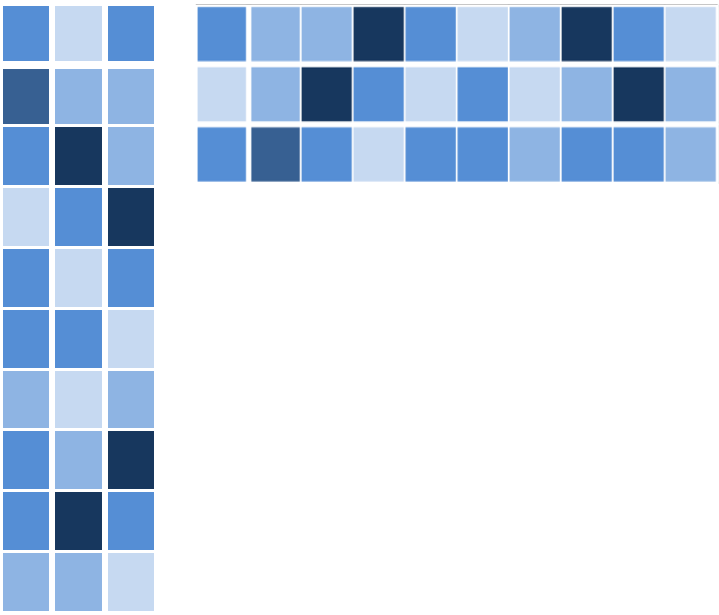
\includegraphics[width=0.65\textwidth]{\LectureFigs/rankr_matrix.pdf} \\
	\vspace{0.3em}
	unknown rank-$r$ matrix $\bm{\Theta}^{\star}\in \mathbb{R}^{d \times d}$
\end{center}
\end{column}


\begin{column}{0.45\textwidth}  
\begin{center}
\vspace{-2.5em}
\[
 \begin{bmatrix}
   {\color{blue} \checkmark} & {\color{red} ?} &{\color{red} ?}  & {\color{red} ?} & {\color{blue} \checkmark} & {\color{red} ?} \\
   {\color{red} ?} & {\color{red} ?} & {\color{blue} \checkmark} & {\color{blue} \checkmark} & {\color{red} ?} & {\color{red} ?} \\
   {\color{blue} \checkmark} & {\color{red} ?} & {\color{red} ?} & {\color{blue} \checkmark} & {\color{red} ?} & {\color{red} ?} \\
   {\color{red} ?} & {\color{red} ?} & {\color{blue} \checkmark}  & {\color{red} ?} &{\color{red} ?}  & {\color{blue} \checkmark} \\
   {\color{blue} \checkmark}  &  {\color{red} ?} & {\color{red} ?} & {\color{red} ?}  & {\color{red} ?} & {\color{red} ?} \\
   {\color{red} ?} & {\color{blue} \checkmark} &{\color{red} ?}  & {\color{red} ?} & {\color{blue} \checkmark} & {\color{red} ?} \\
   {\color{red} ?}  &{\color{red} ?} & {\color{blue} \checkmark} &
   {\color{blue} \checkmark} & {\color{red} ?} & {\color{red} ?}
\end{bmatrix}
\]
 \\
 sampling set $\Omega$
\end{center}
\end{column}


\end{columns}

}

\uncover<2->{
\vfill
\vspace{1em}


{
\setbeamercolor{block body}{bg=babyblueeyes,fg=black}

\begin{varblock}[\textwidth]{}
\vspace{-1.4em}
   \begin{align*}
\text{observations:}\qquad & Y_{i,j}=\Theta_{i,j}^{\star}+  \text{noise},\quad(i,j)\in\Omega \\
	\text{goal:}\qquad & \text{estimate } \bm{\Theta}^{\star} 
\end{align*}
\end{varblock}
}



}
% \uncover<3>{\hfill {\small {\em --- trace regression with} $Y_{i,j} = \mathsf{Tr}(\bm{e}_{j}\bm{e}_{i}^{\top} \bm{\Theta}^{\star} )+ \text{noise}$ }}

	


\end{frame}





\begin{frame}
  \frametitle{Motivation 1: recommendation systems}

\begin{center}
  \begin{center}
\includegraphics[width=0.5\textwidth]{\LectureFigs/NetflixMahdi} \\
%\hfill {\footnotesize\em figure credit: Emmanuel Cand\`es ~~}
\end{center} 

\vspace{1em}
\begin{itemize}
  \itemsep0.3em
  \item Netflix challenge: Netflix provides highly incomplete ratings from nearly 0.5 million users \& 20k movies
  \item How to predict unseen user ratings for movies?
\end{itemize}
\end{center}
\end{frame}


\begin{frame}
\frametitle{In general, we cannot infer missing ratings}


\bigskip

\begin{columns}
\begin{column}{0.5\textwidth}
\[
 \begin{bmatrix}
   {\color{blue} \checkmark} & {\color{red} ?} &{\color{red} ?}  & {\color{red} ?} & {\color{blue} \checkmark} & {\color{red} ?} \\
   {\color{red} ?} & {\color{red} ?} & {\color{blue} \checkmark} & {\color{blue} \checkmark} & {\color{red} ?} & {\color{red} ?} \\
   {\color{blue} \checkmark} & {\color{red} ?} & {\color{red} ?} & {\color{blue} \checkmark} & {\color{red} ?} & {\color{red} ?} \\
   {\color{red} ?} & {\color{red} ?} & {\color{blue} \checkmark}  & {\color{red} ?} &{\color{red} ?}  & {\color{blue} \checkmark} \\
   {\color{blue} \checkmark}  &  {\color{red} ?} & {\color{red} ?} & {\color{red} ?}  & {\color{red} ?} & {\color{red} ?} \\
   {\color{red} ?} & {\color{blue} \checkmark} &{\color{red} ?}  & {\color{red} ?} & {\color{blue} \checkmark} & {\color{red} ?} \\
   {\color{red} ?}  &{\color{red} ?} & {\color{blue} \checkmark} &
   {\color{blue} \checkmark} & {\color{red} ?} & {\color{red} ?}
\end{bmatrix}
\]
\end{column}

\begin{column}{0.5\textwidth}  
\begin{center}
\includegraphics[width=0.9\textwidth]{\LectureFigs/NetflixMahdi} \\
%\hfill {\footnotesize\em figure credit: Emmanuel Cand\`es ~~}
\end{center}
\end{column}

\end{columns}

%\begin{itemize}
%\item 
\bigskip

\begin{center}
Underdetermined system (more unknowns than equations)
\end{center}
%\item Seems hopeless

%\end{itemize}

\end{frame}


\begin{frame}
  \frametitle{... unless rating matrix has some structure} 

\begin{center}
\includegraphics[width=0.9\textwidth]{\LectureFigs/matrix_factorization.jpg} \\
% \hfill {\footnotesize\em adapted from mx's blog}
\end{center}


  \vfill 
  
  \begin{center}
  \alert{low-rank} approximation~$\longrightarrow$~a few factors explain most of  data  
\end{center}


\end{frame}


\begin{frame}
\frametitle{Motivation 2: sensor localization}  

\begin{center}
\includegraphics[width=0.6\textwidth]{\LectureFigs/localization_sensor.png}
\end{center} 
\begin{itemize}

%\item $n$ sensors\,/\,points $\bx_j \in\mathbb{R}^3, ~{j=1,\cdots, n} $
%
\item Observe partial pairwise distances
%\[
%  D_{i,j}= \|\bx_i - \bx_j\|_2^2 = \|\bx_i \|_2^2 + \| \bx_j \|_2^2 - 2 \bx_i^{\top} \bx_j 
%\]
%e.g.  in wireless sensor network, each sensor can measure the distance to its  neighbors, would like to globally locate all sensors.

\item Goal: infer distance between every pair of nodes

\end{itemize}



\end{frame}



\begin{frame}
\frametitle{Motivation 2: sensor localization}

%\begin{itemize}
%\item 
Introduce location matrix
$$\bX =\begin{bmatrix}
- &\bx_1^{\top}  &- \\
- &\bx_2^{\top} &-\\
- &\vdots &- \\
- &\bx_d^{\top} &-
\end{bmatrix} \in\mathbb{R}^{d \times 3}$$
then distance matrix $\bm{D} = [D_{i,j}]_{1\leq i,j\leq d}$ can be written as
%
\[
\bm{D}=\underset{\alertb{\text{low rank}}}{\underbrace{\underset{\alertb{\text{rank 1}}}{\underbrace{\left[\begin{array}{c}
\|\bm{x}_{1}\|_{2}^{2}\\
\vdots\\
\|\bm{x}_{d}\|_{2}^{2}
\end{array}\right]\,\bm{1}^{\top}}}+\underset{\alertb{\text{rank 1}}}{\underbrace{\bm{1}\,\cdot\left[\|\bm{x}_{1}\|_{2}^{2},\cdots,\|\bm{x}_{d}\|_{2}^{2}\right]}}-\underset{\alertb{\text{rank 3}}}{\underbrace{2\bm{X}\bm{X}^{\top}}}}}
\]
%
%\[
% \bm{D} = \underset{\alertb{\text{low rank}}}{\underbrace{ \bm{d}_2 \,\bm{1}^{\top} + \bm{1}\, \bm{d}_2^{\top} - 2\bX \bX^{\top} }}
%\]
%where $\bm{d}_2 :=[\hspace{0.1em}\|\bm{x}_1\|_2^2,\cdots,\|\bm{x}_n\|_2^2\hspace{0.1em}]^{\top}$
%\item $$.% (In $d=3$: $\mbox{rank}(\bM)=3$)
%\end{itemize} 

\vfill

{
\setbeamercolor{block body}{bg=babyblueeyes,fg=black}

\begin{varblock}[\textwidth]{}
   \vspace{-1.5em}
   \begin{center}
     \[
        \text{rank}(\bm{D})  \ll d \quad \longrightarrow \quad  \text{low-rank matrix completion}
     \] 
   \end{center}
\end{varblock}
}


\end{frame}





\begin{frame}
  \frametitle{Least-squares estimator}
  \begin{align*}
    \underset{\bm{\Theta}\in \mathbb{R}^{d \times d}}{\text{minimize}} \qquad &f(\bm{\Theta})=  \sum_{(i,j)\in\Omega} ( \Theta_{i,j} - Y_{i,j} )^{2} \\
    \text{subject to } \qquad &\mathsf{rank}(\bm{\Theta}) = r
  \end{align*}

\pause
  {\hfill \footnotesize \em --- This is also MLE when noise follows Gaussian}

  \pause
  {
\vfill
\vspace{1em}
\setbeamercolor{block body}{bg=babyblueeyes,fg=black}

\begin{varblock}[\textwidth]{}
\centering
   \alert{{\bf Challenge: }}  nonconvexity $\Longrightarrow$ computational hardness
\end{varblock}
}
\end{frame}




\begin{frame}
  \frametitle{Popular workaround: convex relaxation}
  
  
  \begin{center}
    \includegraphics[width=0.75 \textwidth]{\LectureFigs/cvx_relaxation.pdf}
  \end{center}
  
  \vfill
  Relax nonconvex problems into convex ones by finding convex surrogates
  

\end{frame}

\begin{frame}
  \frametitle{Convex relaxation for matrix completion}
  Replace rank constraint by nuclear norm constraint
    \begin{align*}
    \underset{\bm{\Theta}\in \mathbb{R}^{d \times d}}{\text{minimize}} \qquad &f(\bm{\Theta})=  \sum_{(i,j)\in\Omega} ( \Theta_{i,j} - Y_{i,j} )^{2} \\
    \text{subject to } \qquad &\xcancel{\mathsf{rank}(\bm{\Theta}) = r} \quad \alert{\|\bm{\Theta}\|_{*}} \leq t
  \end{align*}

  {\hfill \footnotesize ---~~ $\|\bm{\Theta}\|_* = \sum_{i=1}^{d} \sigma_{i}(\bm{\Theta})$  }

\vfill

\pause
  {
\setbeamercolor{block body}{bg=babyblueeyes,fg=black}

\begin{varblock}[\textwidth]{}
\textbf{convex relaxation (regularized version):}
  \vspace{-2em}
\begin{center}
\[
   \underset{\bm{\Theta}\in\mathbb{R}^{d\times d}}{\text{minimize}}\quad  \sum_{(i,j)\in\Omega}\big(\Theta_{i,j}-Y_{i,j}\big)^{2}  +\lambda{\|\bm{\Theta}\|_{*}}
\]  
\end{center}
\end{varblock}
}
\end{frame}

\begin{frame}
\frametitle{Convex relaxation: pros and cons}


  {
\setbeamercolor{block body}{bg=babyblueeyes,fg=black}

\begin{varblock}[\textwidth]{}
\textbf{convex relaxation (regularized version):}
  \vspace{-2em}
\begin{center}
\[
   \underset{\bm{\Theta}\in\mathbb{R}^{d\times d}}{\text{minimize}}\quad  \sum_{(i,j)\in\Omega}\big(\Theta_{i,j}-Y_{i,j}\big)^{2}  +\lambda{\|\bm{\Theta}\|_{*}}
\]  
\end{center}
\end{varblock}
}

{
\vfill
\vspace{1em}
\setbeamercolor{block body}{bg=babyblueeyes,fg=black}

\begin{varblock}[\textwidth]{}
\centering
    \alertb{\bf Pro:} often achieve statistical optimality \\ \pause
   \alert{{\bf Issue: }}  expensive in computation/memory
\end{varblock}
}
%\alert{not every problem has a natural convex relxation}

\end{frame}



\begin{frame}[plain]
  
\vfill

\centering
  {\Large\em Can we solve matrix completion with lower computational cost?}
  
\vfill

\end{frame}




\begin{frame}
  \frametitle{Spectral methods}

  \begin{itemize}
  \item Assumption: each entry is observed indep. with probability $p$ \pause
  \item Key observation: let
  \[
  \hat Y_{i,j} = \begin{cases} \frac{1}{p} Y_{i,j},\qquad & \text{if }(i,j) \text{ is observed}, \\
  0,\qquad & \text{otherwise}
  \end{cases}
  \]

  we have $\mathbb{E} [ \hat{\bm{Y}} ] = \bm{\Theta}^{\star}$
  \end{itemize}

  \pause
  \vfill
  {
\setbeamercolor{block body}{bg=babyblueeyes,fg=black}

\begin{varblock}[\textwidth]{}
\textbf{spectral method:} \\
\begin{center}
deploy best rank-$r$ approximation to $\hat{\bm{Y}}$ as estimator of $\bm{\Theta}^{\star}$
\end{center}
  \end{varblock}
}

\pause
\hfill --- simple, but sometimes statistically inefficient 
\end{frame}



\begin{frame}
\frametitle{Nonconvex optimization}

\bigskip

  Represent low-rank matrix by $\bm{L}\bm{R}^{\top}$ with $\underset{\alert{\text{low-rank factors}}}{\underbrace{\bm{L},\bm{R}\in \mathbb{R}^{d\times r}}}$ 


\begin{figure}
  \includegraphics[width=0.35\textwidth]{\LectureFigs/XY_factor-plain.pdf}
\end{figure}

\vfill
{
\setbeamercolor{block body}{bg=babyblueeyes,fg=black}


\begin{varblock}[\textwidth]{}
\[
  \underset{\bm{L},\bm{R}\in \mathbb{R}^{d\times r}}{\text{minimize}}~~ f(\bm{L},\bm{R})=  \sum_{(i,j)\in\Omega}\Big[ \big( \bm{L}\bm{R}^{\top} \big)_{i,j} - Y_{i,j} \Big]^{2} 
\]  
\end{varblock}
}

%\alert{linear model after fixing $\bm{L}$}

\end{frame}




\begin{frame}
\frametitle{Two-stage algorithm}

\vspace{-1em}
\[
  \underset{\bm{L},\bm{R}\in \mathbb{R}^{d\times r}}{\text{minimize}}~~ f(\bm{L},\bm{R})= \sum_{(i,j)\in\Omega}\Big[ \big( \bm{L}\bm{R}^{\top} \big)_{i,j} - Y_{i,j} \Big]^{2}
\]


\pause
\vspace{-2em}

\begin{columns}
\begin{column}{0.3\textwidth}

\begin{center}
  \includegraphics[width=1.05\textwidth,angle=-40]{\LectureFigs/GD2.png}
\end{center}

\end{column}



\begin{column}{0.7\textwidth}

\begin{itemize}
\itemsep 1em
\item {\bf spectral initialization:}  $(\bm{L}^{0}, \bm{R}^0)$ 
  
  \quad --- top singular vectors of $\hat{\bm{Y}}$
  %\alert{inverse probability weighting}
  %\[
  %\frac{1}{m}\sum_{i=1}^{m}(\bm{a}_{i}^{\top}\bm{a}^{\star})^{2}\bm{a}_{i}\bm{a}_{i}^{\top}
  %\]
%\pause
\item {\bf gradient descent:} for $t=0,1,\ldots $

\vspace{-1.5em}
\begin{align*}
  \bm{L}^{t+1}&= \bm{L}^t- \eta_t \, \nabla_{\bm{L}} f(\bm{L}^t, \bm{R}^t) \\ 
  \bm{R}^{t+1}&= \bm{R}^t- \eta_t \, \nabla_{\bm{R}} f(\bm{L}^t, \bm{R}^t)
\end{align*}
%
\end{itemize}

\end{column}
\end{columns}

\pause
\vspace{-1em}
{
\setbeamercolor{block body}{bg=babyblueeyes,fg=black}

\begin{varblock}[\textwidth]{}
\begin{center}
nonconvex estimator achieves optimal estimation error
\end{center}
\end{varblock}
\hfill {\em \small --- Ma, Wang, Chi, Chen~'17}
}





\end{frame}

% \begin{frame}
% \frametitle{Main theme of this course}

% \begin{itemize}
%   \itemsep1em
%   \item Low-dimensional structure (e.g.~sparsity, low rank)
%   \pause
%   \item Incoherent sensing mechanism (often designed via ``random'' sampling)
%   \pause
%   \item Efficient algorithms (convex, nonconvex, ...)
% \end{itemize}


% \vfill
% \pause

% \begin{center}
%   {\em We can estimate many low-dimensional structures of interest from
%     highly incomplete data by efficient algorithms}
% \end{center}

% \vfill

% \end{frame}


\begin{frame}
  \frametitle{Main theme of this course}

  By blending \alertb{statistical} and \alertb{computational} theory, we can extract useful information from big data more efficiently
\vfill
  \begin{center}
    \includegraphics[width=\textwidth]{\LectureFigs/opt_Stat.pdf}
\end{center}


\end{frame}


\begin{frame}
\frametitle{Tentative topics}

\begin{itemize}
  \item Spectral methods
    \begin{itemize}
      \item Classic $\ell_2$ matrix perturbation theory
      \item Matrix concentration inequalities
      \item Applications of spectral methods ($\ell_2$ theory)
      \item $\ell_{\infty}$ matrix perturbation theory
      \item Applications of spectral methods ($\ell_{\infty}$ theory)
    \end{itemize}
  \item Nonconvex optimization
    \begin{itemize}
      \item Basic optimization theory
      \item Generic local analysis for regularized gradient descent (GD)
      \item Refined local analysis for vanilla GD
      \item Global landscape analysis
      \item Gradient descent with random initialization
    \end{itemize}
  \item Convex relaxation
    \begin{itemize}
      \item Compressed sensing and sparse recovery
      \item Phase transition and convex geometry
      % \item Week 8: Gaussian graphical models and graphical lasso
      \item Low-rank matrix recovery
      \item Robust principal component analysis
      % \item Week 10: Nonconvex matrix factorization
    \end{itemize}
  % \item Week 12: Learning shallow neural networks
\end{itemize}

\end{frame}




\begin{frame}[plain]

\vfill
\begin{center}
  {\Large\bf Logistics}
\end{center}
\vfill

\end{frame}


\begin{frame}
\frametitle{Why you \alert{should not} take this course}


\begin{itemize}
  \itemsep1em
  \item<2-> There will be quite a few THEOREMS and PROOFS ...
  \pause
  \item<3-> Nonrigorous/heuristic arguments from time to time
  %\pause
  %\item<4-> Taught for the first time
\end{itemize}

\end{frame}






\begin{frame}
\frametitle{Why you \alert{should} consider taking this course}


\begin{itemize}
  \itemsep1em
  \item<2-> There will be quite a few THEOREMS and PROOFS ...
  \begin{itemize}
    \item<3-> promote deeper understanding of scientific results
  \end{itemize}
  
  \item<4-> Nonrigorous/heuristic arguments from time to time
  \begin{itemize}
    \vspace{0.5em}
    \item<5-> ``nonrigorous'' but grounded in rigorous theory
    \item<5-> help develop intuition
  \end{itemize}
  
  %\item<6-> Taught for the first time
  %\begin{itemize}
  %  \item<7-> We need your feedback!
  %\end{itemize}
\end{itemize}

\end{frame}

\begin{frame}
\frametitle{Prerequisites}



\begin{itemize}
  \itemsep0.5em
  \item linear algebra 
  \item probability theory
  \item a programming language (e.g., Matlab, Python, Julia, $\ldots$)
  \item {\em knowledge in convex optimization}
\end{itemize}



\end{frame}


\begin{frame}
\frametitle{Textbooks}

We recommend these  books, but will not follow them closely

\begin{columns}
  \begin{column}{0.32\textwidth}
  \begin{center}
    \includegraphics[width=0.8\textwidth]{high-dim-stats-Wainwright.jpg}
  \end{center}


  \end{column} 

  \begin{column}{0.32\textwidth}
  \begin{center}
     \includegraphics[width=0.8\textwidth]{high-dim-prob-Vershynin.jpg}
  \end{center}

  \end{column}

  \begin{column}{0.32\textwidth}
  \begin{center}

	%Statistical machine learning for high-dimensional data, J.~Fan, R.~Li, C.~Zhang, H.~Zou \\
    \includegraphics[width=0.76\textwidth]{jianqing-book.jpeg}
  \end{center} 

  \end{column} 


\end{columns}

\end{frame}

\begin{frame}
  \frametitle{Useful references}

\begin{itemize}
  \item {\textit{Spectral Methods for Data Science: A Statistical Perspective}},  Yuxin Chen, Yuejie Chi, Jianqing Fan, and Cong Ma 
\item {\textit{Nonconvex optimization meets low-rank matrix factorization: An overview}},  Yuejie Chi, Yue M.~Lu, and Yuxin Chen 
% \item {\textit{Introduction to the non-asymptotic analysis of random matrices}}, Roman Vershynin
\item {\textit{Convex optimization}}, Stephen Boyd, and Lieven Vandenberghe
% \item {\textit{Topics in random matrix theory}}, Terence Tao

\end{itemize} 
\end{frame}





\begin{frame}
\frametitle{Grading}


\begin{itemize}
\itemsep3em

\item Homework: ${\sim}$3 problem sets involving proofs and simulations
\smallskip
\begin{itemize}
  \itemsep0.3em
  % \item Use \alert{Piazza} as the main mode of electronic communication; please post (and answer) questions there!
  \item Due at Thursday lectures
\end{itemize}



\item Course project 
\begin{itemize}
  \item Either individually or in groups of two
\end{itemize}


\item Your grade: $\max\{ 0.4\times \text{HW} + 0.6\times \text{project},\, \text{project} \}$ 

\end{itemize}


\end{frame}


\begin{frame}
\frametitle{Course project}

Two forms
\begin{itemize}
\itemsep0.5em
\item literature review
\item original research
\begin{itemize}
  \item \alert{\em You are strongly encouraged to combine it with your own research}
\end{itemize}
\end{itemize}

\pause
\vfill

Three milestones

\begin{itemize}
\itemsep0.5em
\item proposal (due Oct.~21st): up to 1 page
\item in-class presentation: last week of class
\item report (due TBA): up to 4 pages with unlimited appendix
\end{itemize}


\end{frame}



% \begin{frame}
% \frametitle{Asymptotic notation used in this course}

% \begin{itemize}
%    \itemsep1em
%    \item  $f(n) \lesssim g(n)$ or $f(n) = O(g(n))$ means 
%    \[
%      \lim_{n\rightarrow\infty} \frac{|f(n)|}{|g(n)|} ~\leq~ \text{const} 
%    \]
%    \item  $f(n) \gtrsim g(n)$ or $f(n) = \Omega(g(n))$ means 
%    \[
%      \lim_{n\rightarrow\infty} \frac{|f(n)|}{|g(n)|} ~\geq~ \text{const} 
%    \]
%    \item  $f(n) \asymp g(n)$ or $f(n) = \Theta(g(n))$ means 
%    \[
%       \text{const}_1 ~\leq~ \lim_{n\rightarrow\infty} \frac{|f(n)|}{|g(n)|} ~\leq~ \text{const}_2 
%    \]


%    \item  $f(n) = o(g(n))$ means 
%    \[
%        \lim_{n\rightarrow\infty} \frac{|f(n)|}{|g(n)|} ~=~ 0
%    \]

% \end{itemize}

% \end{frame}


% \begin{frame}
% \frametitle{Reference}

% {\small
% \begin{itemize} 
%   \itemsep0.5em
%   \item ``{\textit{Mathematics of sparsity (and a few other things)}},'' E.~Candes, {\textit{International Congress of Mathematicians}}, 2014.
%   \item ``{\textit{Statistical learning with sparsity: the Lasso and generalizations}},'' T.~Hastie, R.~Tibshirani, and M.~Wainwright,  2015.
% \end{itemize}
% }

% \end{frame}








\end{document}

